%% Package and Class "uiucthesis2014" for use with LaTeX2e.
\documentclass[edeposit,fullpage,12pt]{uiucthesis2018}


\usepackage[acronym,toc]{glossaries}
%\newacronym{<++>}{<++>}{<++>}
\newacronym[longplural={metric tons of heavy metal}]{MTHM}{MTHM}{metric ton of heavy metal}
\newacronym{ABM}{ABM}{agent-based modeling}
\newacronym{ACDIS}{ACDIS}{Program in Arms Control \& Domestic and International Security}
\newacronym{AHTR}{AHTR}{Advanced High Temperature Reactor}
\newacronym{ANDRA}{ANDRA}{Agence Nationale pour la gestion des D\'echets RAdioactifs, the French National Agency for Radioactive Waste Management}
\newacronym{ANL}{ANL}{Argonne National Laboratory}
\newacronym{API}{API}{application programming interface}
\newacronym{ARE}{ARE}{Aircraft Reactor Experiment}
\newacronym{ASME}{ASME}{American Society of Mechanical Engineers}
\newacronym{ATWS}{ATWS}{Anticipated Transient Without Scram}
\newacronym{BDBE}{BDBE}{Beyond Design Basis Event}
\newacronym{BIDS}{BIDS}{Berkeley Institute for Data Science}
\newacronym{CAFCA}{CAFCA}{ Code for Advanced Fuel Cycles Assessment }
\newacronym{CDTN}{CDTN}{Centro de Desenvolvimento da Tecnologia Nuclear}
\newacronym{CEA}{CEA}{Commissariat \`a l'\'Energie Atomique et aux \'Energies Alternatives}
\newacronym{CFD}{CFD}{Computational Fluid Dynamics}
\newacronym{CI}{CI}{continuous integration}
\newacronym{CNEN}{CNEN}{Comiss\~{a}o Nacional de Energia Nuclear}
\newacronym{CNERG}{CNERG}{Computational Nuclear Engineering Research Group}
\newacronym{CNRS}{CNRS}{Centre National de la Recherche Scientifique, the French National Centre for Scientific Research}
\newacronym{COMSOL}{COMSOL}{COMmon SOLution}
\newacronym{COSI}{COSI}{Commelini-Sicard}
\newacronym{COTS}{COTS}{commercial, off-the-shelf}
\newacronym{CSNF}{CSNF}{commercial spent nuclear fuel}
\newacronym{CTAH}{CTAHs}{Coiled Tube Air Heaters}
\newacronym{CUBIT}{CUBIT}{CUBIT Geometry and Mesh Generation Toolkit}
\newacronym{CURIE}{CURIE}{Centralized Used Fuel Resource for Information Exchange}
\newacronym{DAG}{DAG}{directed acyclic graph}
\newacronym{DANESS}{DANESS}{Dynamic Analysis of Nuclear Energy System Strategies}
\newacronym{DBE}{DBE}{Design Basis Event}
\newacronym{DESAE}{DESAE}{Dynamic Analysis of Nuclear Energy Systems Strategies}
\newacronym{DHS}{DHS}{Department of Homeland Security}
\newacronym{DNP}{DNP}{delayed neutron precursor}
\newacronym{DOE}{DOE}{Department of Energy}
\newacronym{DMSR}{DMSR}{Denatured Molten Salt Reactor}
\newacronym{DRACS}{DRACS}{Direct Reactor Auxiliary Cooling System}
\newacronym{DRE}{DRE}{dynamic resource exchange}
\newacronym{DSNF}{DSNF}{DOE spent nuclear fuel}
\newacronym{DYMOND}{DYMOND}{Dynamic Model of Nuclear Development }
\newacronym{EBS}{EBS}{Engineered Barrier System}
\newacronym{EDZ}{EDZ}{Excavation Disturbed Zone}
\newacronym{EPA}{EPA}{Environmental Protection Agency}
\newacronym{EP}{EP}{Engineering Physics}
\newacronym{EVOL}{EVOL}{Evaluation and Viability of Liquid Fuel Fast Reactor System}
\newacronym{FCO}{FCO}{Fuel Cycle Options}
\newacronym{FCT}{FCT}{Fuel Cycle Technology}
\newacronym{FEHM}{FEHM}{Finite Element Heat and Mass Transfer}
\newacronym{FEPs}{FEPs}{Features, Events, and Processes}
\newacronym{FHR}{FHR}{Fluoride-Salt-Cooled High-Temperature Reactor}
\newacronym{FLiBe}{FLiBe}{Fluoride-Lithium-Beryllium}
\newacronym{FP}{FP}{fission product}
\newacronym{GDSE}{GDSE}{Generic Disposal System Environment}
\newacronym{GDSM}{GDSM}{Generic Disposal System Model}
\newacronym{GENIUSv1}{GENIUSv1}{Global Evaluation of Nuclear Infrastructure Utilization Scenarios, Version 1}
\newacronym{GENIUSv2}{GENIUSv2}{Global Evaluation of Nuclear Infrastructure Utilization Scenarios, Version 2}
\newacronym{GENIUS}{GENIUS}{Global Evaluation of Nuclear Infrastructure Utilization Scenarios}
\newacronym{GIF}{GIF}{Generation IV International Forum}
\newacronym{GPAM}{GPAM}{Generic Performance Assessment Model}
\newacronym{GRSAC}{GRSAC}{Graphite Reactor Severe Accident Code}
\newacronym{GUI}{GUI}{graphical user interface}
\newacronym{HALEU}{HALEU}{high-assay low-enriched uranium}
\newacronym{HLW}{HLW}{high level waste}
\newacronym{HPC}{HPC}{high-performance computing}
\newacronym{HTC}{HTC}{high-throughput computing}
\newacronym{HTGR}{HTGR}{High Temperature Gas-Cooled Reactor}
\newacronym{IAEA}{IAEA}{International Atomic Energy Agency}
\newacronym{IEMA}{IEMA}{Illinois Emergency Mangament Agency}
\newacronym{IHLRWM}{IHLRWM}{International High Level Radioactive Waste Management}
\newacronym{INL}{INL}{Idaho National Laboratory}
\newacronym{IPRR1}{IRP-R1}{Instituto de Pesquisas Radioativas Reator 1}
\newacronym{IRP}{IRP}{Integrated Research Project}
\newacronym{ISFSI}{ISFSI}{Independent Spent Fuel Storage Installation}
\newacronym{ISRG}{ISRG}{Independent Student Research Group}
\newacronym{JFNK}{JFNK}{Jacobian-Free Newton Krylov}
\newacronym{LANL}{LANL}{Los Alamos National Laboratory}
\newacronym{LBNL}{LBNL}{Lawrence Berkeley National Laboratory}
\newacronym{LCOE}{LCOE}{levelized cost of electricity}
\newacronym{LDRD}{LDRD}{laboratory directed research and development}
\newacronym{LEU}{LEU}{low-enriched uranium}
\newacronym{LFR}{LFR}{Lead-Cooled Fast Reactor}
\newacronym{LLNL}{LLNL}{Lawrence Livermore National Laboratory}
\newacronym{LMFBR}{LMFBR}{Liquid Metal Fast Breeder Reactor}
\newacronym{LOFC}{LOFC}{Loss of Forced Cooling}
\newacronym{LOHS}{LOHS}{Loss of Heat Sink}
\newacronym{LOLA}{LOLA}{Loss of Large Area}
\newacronym{LP}{LP}{linear program}
\newacronym{LWR}{LWR}{Light Water Reactor}
\newacronym{MAGNOX}{MAGNOX}{Magnesium Alloy Graphie Moderated Gas Cooled Uranium Oxide Reactor}
\newacronym{MA}{MA}{minor actinide}
\newacronym{MCFR}{MCFR}{Molten Chloride Fast Reactor}
\newacronym{MCNP}{MCNP}{Monte Carlo N-Particle code}
\newacronym{MILP}{MILP}{mixed-integer linear program}
\newacronym{MIT}{MIT}{the Massachusetts Institute of Technology}
\newacronym{MOAB}{MOAB}{Mesh-Oriented datABase}
\newacronym{MOOSE}{MOOSE}{Multiphysics Object-Oriented Simulation Environment}
\newacronym{MOSART}{MOSART}{Molten Salt Actinide Recycler and Transmuter}
\newacronym{MOX}{MOX}{mixed oxide}
\newacronym{MPI}{MPI}{Message Passing Interface}
\newacronym{MRPP}{MRPP}{Multiregion Processing Plant}
\newacronym{MSBR}{MSBR}{Molten Salt Breeder Reactor}
\newacronym{MSFR}{MSFR}{Molten Salt Fast Reactor}
\newacronym{MSRE}{MSRE}{Molten Salt Reactor Experiment}
\newacronym{MSR}{MSR}{Molten Salt Reactor}
\newacronym{NAGRA}{NAGRA}{National Cooperative for the Disposal of Radioactive Waste}
\newacronym{NEAMS}{NEAMS}{Nuclear Energy Advanced Modeling and Simulation}
\newacronym{NEUP}{NEUP}{Nuclear Energy University Programs}
\newacronym{NFCSim}{NFCSim}{Nuclear Fuel Cycle Simulator}
\newacronym{NGNP}{NGNP}{Next Generation Nuclear Plant}
\newacronym{NMWPC}{NMWPC}{Nuclear MW Per Capita}
\newacronym{NNSA}{NNSA}{National Nuclear Security Administration}
\newacronym{NPP}{NPP}{Nuclear Power Plant}
\newacronym{NPRE}{NPRE}{Department of Nuclear, Plasma, and Radiological Engineering}
\newacronym{NQA1}{NQA-1}{Nuclear Quality Assurance - 1}
\newacronym{NRC}{NRC}{Nuclear Regulatory Commission}
\newacronym{NSF}{NSF}{National Science Foundation}
\newacronym{NSSC}{NSSC}{Nuclear Science and Security Consortium}
\newacronym{NUWASTE}{NUWASTE}{Nuclear Waste Assessment System for Technical Evaluation}
\newacronym{NWF}{NWF}{Nuclear Waste Fund}
\newacronym{NWTRB}{NWTRB}{Nuclear Waste Technical Review Board}
\newacronym{OCRWM}{OCRWM}{Office of Civilian Radioactive Waste Management}
\newacronym{ORION}{ORION}{ORION}
\newacronym{ORNL}{ORNL}{Oak Ridge National Laboratory}
\newacronym{PARCS}{PARCS}{Purdue Advanced Reactor Core Simulator}
\newacronym{PBAHTR}{PB-AHTR}{Pebble Bed Advanced High Temperature Reactor}
\newacronym{PBFHR}{PB-FHR}{Pebble-Bed Fluoride-Salt-Cooled High-Temperature Reactor}
\newacronym{PDE}{PDE}{partial differential equation}
\newacronym{PEI}{PEI}{Peak Environmental Impact}
\newacronym{PH}{PRONGHORN}{PRONGHORN}
\newacronym{PRIS}{PRIS}{Power Reactor Information System}
\newacronym{PRKE}{PRKE}{Point Reactor Kinetics Equations}
\newacronym{PSPG}{PSPG}{Pressure-Stabilizing/Petrov-Galerkin}
\newacronym{PWAR}{PWAR}{Pratt and Whitney Aircraft Reactor}
\newacronym{PWR}{PWR}{Pressurized Water Reactor}
\newacronym{PyNE}{PyNE}{Python toolkit for Nuclear Engineering}
\newacronym{PyRK}{PyRK}{Python for Reactor Kinetics}
\newacronym{QA}{QA}{quality assurance}
\newacronym{RDD}{RD\&D}{Research Development and Demonstration}
\newacronym{RD}{R\&D}{Research and Development}
\newacronym{REE}{REE}{rare earth element}
\newacronym{RELAP}{RELAP}{Reactor Excursion and Leak Analysis Program}
\newacronym{RIA}{RIA}{Reactivity Insertion Accident}
\newacronym{RIF}{RIF}{Region-Institution-Facility}
\newacronym{ROD}{ROD}{Reactor Optimum Design}
\newacronym{SAMOFAR}{SAMOFAR}{Safety Assessment of the Molten Salt Fast Reactor}
\newacronym{SAM}{SAM}{System Analysis Module}
\newacronym{SFR}{SFR}{Sodium-Cooled Fast Reactor}
\newacronym{SINDAG}{SINDA{\textbackslash}G}{Systems Improved Numerical Differencing Analyzer $\backslash$ Gaski}
\newacronym{SKB}{SKB}{Svensk K\"{a}rnbr\"{a}nslehantering AB}
\newacronym{SNF}{SNF}{spent nuclear fuel}
\newacronym{SNL}{SNL}{Sandia National Laboratory}
\newacronym{STC}{STC}{specific temperature change}
\newacronym{SUPG}{SUPG}{Streamline-Upwind/Petrov-Galerkin}
\newacronym{SWF}{SWF}{Separations and Waste Forms}
\newacronym{SWU}{SWU}{Separative Work Unit}
\newacronym{TRIGA}{TRIGA}{Training Research Isotope General Atomic}
\newacronym{TRISO}{TRISO}{Tristructural Isotropic}
\newacronym{TRU}{TRU}{transuranic}
\newacronym{TSM}{TSM}{Total System Model}
\newacronym{TSPA}{TSPA}{Total System Performance Assessment for the Yucca Mountain License Application}
\newacronym{ThOX}{ThOX}{thorium oxide}
\newacronym{UFD}{UFD}{Used Fuel Disposition}
\newacronym{UML}{UML}{Unified Modeling Language}
\newacronym{UOX}{UOX}{uranium oxide}
\newacronym{UQ}{UQ}{uncertainty quantification}
\newacronym{US}{US}{United States}
\newacronym{UW}{UW}{University of Wisconsin}
\newacronym{VISION}{VISION}{the Verifiable Fuel Cycle Simulation Model}
\newacronym{VVER}{VVER}{Voda-Vodyanoi Energetichesky Reaktor (Russian Pressurized Water Reactor)}
\newacronym{VV}{V\&V}{verification and validation}
\newacronym{WIPP}{WIPP}{Waste Isolation Pilot Plant}
\newacronym{YMR}{YMR}{Yucca Mountain Repository Site}
\newacronym{BOL}{BOL}{Beginning-of-Life}
\newacronym{ULOF}{ULOF}{Unprotected Loss of Flow}
\newacronym{LOSCA}{LOSCA}{Loss of Secondary Cooling Accident}
\newacronym{ULOHS}{ULOHS}{Unprotected Loss of Heat Sink}


\usepackage{xspace}
\usepackage{graphics}
\graphicspath{{images/}}

\usepackage{placeins}
\usepackage{booktabs} % nice rules (thick lines) for tables
\usepackage{microtype} % improves typography for PDF

\usepackage[hyphens]{url}
\usepackage{hyperref}
\usepackage{subfig}
\usepackage{hhline}
\usepackage{amsmath}
\usepackage{color}
\usepackage{multirow}
\usepackage{siunitx}
\sisetup{
    input-decimal-markers = .,input-ignore = {,},table-number-alignment = right,
    group-separator={,}, group-four-digits = true
}
\usepackage{fourier}
\usepackage{booktabs}
\newcommand\tab[1][1cm]{\hspace*{#1}}

\usepackage{threeparttable, tablefootnote}

%tikzpicture fit to page width
\usepackage{environ}
\makeatletter
\newsavebox{\measure@tikzpicture}
\NewEnviron{scaletikzpicturetowidth}[1]{%
  \def\tikz@width{#1}%
  \def\tikzscale{1}\begin{lrbox}{\measure@tikzpicture}%
  \BODY
  \end{lrbox}
  \pgfmathparse{#1/\wd\measure@tikzpicture}%
  \edef\tikzscale{\pgfmathresult}%
  \BODY
}

\usepackage{tabularx}
\newcolumntype{b}{>{\hsize=1.0\hsize}X}
\newcolumntype{q}{>{\hsize=0.5\hsize}X}
\newcolumntype{R}{>{\raggedleft\arraybackslash\hsize=0.5\hsize}X}
\newcolumntype{z}{>{\hsize=0.75\hsize}X}
\newcolumntype{s}{>{\hsize=.5\hsize}X}
\newcolumntype{m}{>{\hsize=.75\hsize}X}

\usepackage{cleveref}
\usepackage{datatool}
\usepackage[numbers]{natbib}
\usepackage{notoccite}


\usepackage{tikz}
\usetikzlibrary{positioning, arrows, decorations, shapes}

\usetikzlibrary{shapes.geometric,arrows}
\tikzstyle{process} = [rectangle, rounded corners, minimum width=2.5cm, minimum height=1cm,text centered, draw=black, fill=blue!30]

\tikzstyle{object} = [ellipse, rounded corners, minimum width=3cm, minimum height=1cm,text centered, draw=black, fill=green!30]
\tikzstyle{objectr} = [ellipse, rounded corners, minimum width=3cm, minimum height=1cm,text centered, draw=black, fill=red!30]

\tikzstyle{empty} =  [rectangle, rounded corners, minimum width=2.5cm, minimum height=0.7cm,text centered, draw=black, fill=white!30]
\tikzstyle{arrow} = [thick,->,>=stealth]


\title{Thesis Title}
\author{Sun Myung Park}
\department{Nuclear, Plasma, Radiological Engineering}
%\schools{B.S., National University of Singapore, 2017}
\msthesis
\advisor{Kathryn D. Huff}
\degreeyear{2019}
\committee{Assistant Professor Kathryn D. Huff, Adviser \\ Professor xyz}


\begin{document}
\maketitle

\frontmatter
%% Create an abstract that can also be used for the ProQuest abstract.
%% Note that ProQuest truncates their abstracts at 350 words.
\begin{abstract}

Abstract.

\end{abstract}

\chapter*{Acknowledgments}

Acks.

%% The thesis format requires the Table of Contents to come
%% before any other major sections, all of these sections after
%% the Table of Contents must be listed therein (i.e., use \chapter,
%% not \chapter*).  Common sections to have between the Table of
%% Contents and the main text are:
%%
%% List of Tables
%% List of Figures
%% List Symbols and/or Abbreviations
%% etc.

\tableofcontents
\listoftables
\listoffigures

%% Create a List of Abbreviations. The left column
%% is 1 inch wide and left-justified
%\chapter{List of Abbreviations}
%\printglossaries
%% Create a List of Symbols. The left column
%% is 0.7 inch wide and centered

\pagebreak
\mainmatter

\chapter{Introduction}
\section{Background and Motivation}

Greenhouse gas emission from human activities is the main cause of climate
change, which has dire
consequences on human health and safety due to extreme weather events and the
overall impact on food production \cite{mcmichael_global_2004}.
Electricity generation from burning fossil fuels represents the
greatest source of CO$_2$ emissions (38\% in 2018 \cite{iea_global_2019});
replacing it with low-carbon
alternatives would curb a significant fraction of emissions. Nuclear power is
a viable low-carbon replacement for burning fossil fuels and it provides
consistent base-load power independent of weather and geographical location
\cite{petti_future_2018}. Furthermore, employing a diverse mix of nuclear
power and renewable sources ensures energy security and reliability in our
transition towards a low-carbon future \cite{petti_future_2018}.

The world would have to ramp up the current rate of reactor deployments to
displace a portion of the presently large share of energy production from
fossil
fuel power plants. However, several obstacles stand in the way of mass reactor
deployments. These obstacles include perceived safety risks, sustainability
concerns, nuclear proliferation
risks, and the ability to compete economically with other sources of energy
\cite{massachusetts_institute_of_technology_future_2003}. A potential solution
to the aforementioned issues is the \gls{MSR} concept, one of six advanced
reactor designs selected by the Generation IV International Forum
\cite{gif_technology_2002} for continued research and development.

The primary coolants in MSRs consist of molten salt mixtures
with fissile and/or fertile material dissolved directly in the coolants.
MSRs possess an inherently robust safety feature in the strongly negative fuel
temperature coefficient of reactivity. Some designs can also incorporate the
thorium fuel cycle for improved sustainability arising from the use of
abundant natural thorium resources and reduced transuranic waste. The
latter also reduces economical costs
associated with long-term nuclear waste storage. In addition, the ability to
operate at near atmospheric pressures eliminates the need for a thick pressure
vessel and drives down construction costs, while online fuel reprocessing
reduces reactor downtime during reactor operation.

However, the liquid fuel form also brings about novel computational
challenges in simulating the transient behavior of \glspl{MSR}; the
interactions between neutronics and thermal-hydraulics are stronger due
to greater fuel material expansion. Furthermore, fissile material and
\glspl{DNP} in \glspl{MSR} can flow freely within the primary coolant
loop as opposed to being held in place in a solid fuel matrix. Therefore,
the choice of coupling methods for each set of physics requires careful
consideration. 

Most reactor analysis applications are usually reactor-specific by
design such as TRACE \cite{nrc_trace_nodate} for \glspl{LWR}, and
SAS4A/SASSYS-1 \cite{fanning_sas4a/sassys-1_2017} for
liquid metal cooled reactors. Thus, these applications would disregard
\gls{MSR}-specific phenomena and are inappropriate for \gls{MSR}
analysis without modifications to the source code. Some research efforts
do focus on adapting these applications for \gls{MSR} analysis. Examples
include the coupling of modified versions of TRACE and PARCS
\cite{pettersen_coupled_2016}, and the development of VERA-MSR from the
integrated \gls{LWR} simulation tool VERA \cite{graham_development_2019}.
Others developed their \gls{MSR} simulation tools from general
multiphysics or \gls{CFD} applications such as COMSOL
\cite{fiorina_modelling_2014} and OpenFOAM \cite{aufiero_development_2014}.

Similarly, Moltres \cite{lindsay_introduction_2018} is an open-source MSR
simulation tool built in the \gls{MOOSE} \cite{gaston_physics-based_2015}
parallel finite element framework. Lindsay et al.
\cite{lindsay_introduction_2018} first presented the tool in 2017 and
demonstrated its capabilities by simulating 2-D and 3-D models of the
\gls{MSRE}. The results showed good qualitative
agreement with the original design calculations by \gls{MSRE} researchers at
\gls{ORNL}. This thesis presents some of the new developments in Moltres
allowing for more complex and accurate \gls{MSR} simulations.

\section{Objectives}

This thesis demonstrates latest capabilities of Moltres
\cite{lindsay_introduction_2018}.
In particular, this thesis presents two more recent
developments in Moltres, namely fully integrating \gls{MOOSE}'s incompressible
Navier-Stokes module into Moltres, and introducing a
decay heat model.
The main objective of this thesis is to verify Moltres'
latest capabilities in modeling multiphysics, steady-state, and transient
behavior of fast-spectrum \glspl{MSR} through the study of the \gls{MSFR}
concept. Code-to-code verification is an important exercise in software
development for ensuring that the application produces accurate and reliable
results. This thesis covers the \gls{MSFR} concept mainly because it has been
studied extensively with readily available data in the literature to verify
against. The \gls{MSFR} design also features interesting flow
patterns that greatly affect the steady-state and transient behavior. This
present work will first present a verification of Moltres' \gls{MSFR}
diffusion neutronics against the Monte Carlo neutron transport software
Serpent 2, followed by a verification of
the coupled neutronics/thermal-hydraulics steady-state and accident transient
results against two sets of results published by
Fiorina et al. \cite{fiorina_modelling_2014}. The two sets of results arose
from a collaborative benchmarking exercise by researchers at Politecnico di
Milano and Technical University of Delft with two separate \gls{MSR}
simulation tools. Section \ref{sec:litrev} discusses these tools
in greater detail. The
secondary objective is to identify areas of improvement in Moltres for future
development.

\section{Thesis Outline}

The outline of this thesis is as follows. Chapter 2 discusses the history and
features of \glspl{MSR}, and a literature review of existing \gls{MSR}
simulation tools. The chapter also covers the \gls{MSFR} concept in greater
detail. Chapter 3 details the software and the general modeling
approach for generating the results in this thesis. Chapter 4 provides a
neutronics assessment by comparing key neutronics parameters from Moltres'
eigenvalue calculations to Serpent's Monte Carlo calculations. Chapter 5
presents steady-state results of coupled neutronics/thermal-hydraulics
\gls{MSFR} simulations in Moltres. Chapter 6 presents accident transient
simulation results for unprotected reactivity insertions, unprotected loss of
heat sink, unprotected loss of flow, and unprotected pump overspeed. Lastly,
Chapter 7 summarizes the key findings in this thesis
and posits some potential avenues for future work.


\chapter{Molten Salt Reactors}
\glspl{MSR} are one of six advanced reactor designs shortlisted by
the \gls{GIF} in 2001 for promising significant advances in safety,
sustainability, efficiency, and cost over existing designs in operation
today. This has attracted significant attention and resources towards
\gls{MSR} research, most noticeable by the number of start-up companies that
have emerged in recent years touting various \gls{MSR} designs. This chapter
provides a brief history of \glspl{MSR}, followed by the distinctive features
that earned the concept the label of being a Generation IV reactor. Lastly,
we present the reference specifications of the \gls{MSFR} concept studied in
this work.

\section{History}

The first \gls{MSR}, named the \gls{ARE}, dates back to the 1940s,
as part of the US Aircraft Nuclear Propulsion program; the molten salt
concept was considered due to the stability of molten salts at high
temperatures and neutron radiation. The 2.5
MW$_{\text{th}}$ reactor was built at \gls{ORNL}, where it achieved
criticality on November 1954 and generated 100 MWh over nine days. The fuel
consisted of enriched uranium in a molten salt mixture of NaF, ZrF$_4$, and
UF$_4$, and moderated by blocks of beryllium oxide. The project ultimately
never came to fruition as the development of intercontinental ballistic
missiles effectively eliminated the need for long-range nuclear-powered
bomber aircraft.

However, the successful demonstration of the \gls{ARE} spurred further
research into adapting \glspl{MSR} for civilian power generation. One of the
key findings from the
research was that better economy could be achieved from breeding $^{233}$U
from $^{232}$Th in thermal-spectrum reactors than $^{239}$Pu from $^{238}$U.
Ultimately, these efforts culminated in the \gls{MSRE}, a graphite-moderated
thermal \gls{MSR}.
Although no breeding was attempted with the \gls{MSRE}, scientists at
\gls{ORNL} obtained a wealth of experimental data and new insights from the
study of this reactor. The \gls{MSRE} had a graphite-moderated design with
LiF-BeF$_2$-ZrF$_4$-UF$_4$ fuel salt mixture, initially rated at 10
MW$_{\text{th}}$ but later restricted to 8 MW$_{\text{th}}$ due to a
miscalculation of heat transfer capabilities. 

Design of the \gls{MSRE} commenced in the summer of 1960, with construction
starting in early 1962. The reactor achieved zero-power criticality in June
1965, and 30 days of continuous operation at full power in December 1966.
The reactor operated at full power for the most of the following 15 months,
during which the researchers carried out various experiments. Soon after
shutdown, the $^{235}$U fuel was replaced with $^{233}$U and in January
1969, the \gls{MSRE} became the first reactor to run on $^{233}$U fuel.

Although the \gls{MSRE} was a huge success, \gls{ORNL} failed to secure new
funding for the construction and operation of the \gls{MSBR}. The \gls{MSR}
development program lost out to the competing \gls{LMFBR} program which had
a head start and garnered wider political and technical support.
Nevertheless, from a technical perspective, two independent technology
evaluation and design studies of the \gls{MSR} had ``reported favorably on
the promise of the system".

\section{Features}

As mentioned in the introduction section, the most significant difference
between \glspl{MSR} and other reactor
concepts is the liquid fuel in \glspl{MSR}; fissile and/or fertile material
is dissolved in
high temperature, commonly eutectic mixtures of molten salts. Most \gls{MSR}
designs are circulating-fuel reactors. The primary coolant loop containing
the fuel salt transfers heat through a heat exchanger to the clean,
secondary/intermediate loop.

The flexibility of \glspl{MSR} is best illustrated by the various designs
under development today. Graphite-moderated thermal-spectrum \glspl{MSR} are
typically straight-forward \gls{LEU} burners, or $^{232}$Th/$^{233}$U
breeders, while epithermal- and fast-spectrum \glspl{MSR} have the additional
options of operating as \gls{TRU} fuel burners or $^{238}$U/$^{239}$Pu
breeders. Breeder designs can be further categorized into one- or two-fluid
designs; two-fluid designs feature blanket molten salt mixtures that contain
higher proportions of fertile material than the fuel salt mixture.

\section{Molten Salt Fast Reactor}

The \gls{MSFR} is a reference fast-spectrum \gls{MSR} concept developed
under the \gls{EVOL} and \gls{SAMOFAR} projects. The main reactor
specifications and schematic view are shown in Table * and Fig. *
respectively. Inspired by the \gls{MSBR}, the \gls{MSFR} is
intended to run primarily on a closed thorium fuel cycle with
continuous online fuel reprocessing. Several reasons motivated the omission of
graphite moderators from the \gls{MSFR} design. Graphite is susceptible to
long-term radiation damage and replacement is likely to be necessary during
the operating lifetime of the reactor. The relatively fast neutron spectrum
improves breeding ratios due to higher fission neutron yield in $^{233}$U and
lower parasitic absorption in non-fuel materials. Lastly, graphite has a
positive temperature coefficient of reactivity; eliminating graphite from the
design ensures a greater safety margin.

In the \gls{MSFR} design, fuel salt flows upwards through a 9 m$^3$ central
core region. At the top of the core, the flow separates into 16 smaller
external loops, each of which passes through a heat exchanger before being
pumped back into the bottom of the core. Other instrumentation are situated
along the external loop for online salt reprocessing and gas sparging. The
core is surrounded axially by nickel alloy reflectors, and radially by a
toroidal blanket tank containing fertile salt for breeding. There is a layer
of boron carbide behind the blanket tanks to protect the peripheral equipment
from excessive neutron damage. In case of severe accidents, there is an
actively cooled freeze plug at the bottom of the core that melts when
temperatures exceed a certain threshold. The fuel salt would drain into a
containment vessel designed to keep it subcritical. Reactivity control under
normal operating conditions is performed by varying pump speeds to advantage
of strong thermal feedback. Coupled with the fact that there is no excess
reactivity reserve due to online fuel reprocessing, control rods are not
included in the \gls{MSFR}.

Although the \gls{MSFR} is primarily designed to operate on the thorium fuel
cycle, it can support a range of start-up fuel and feed compositions. This
versatility is particularly important for the first few \glspl{MSFR} to be
deployed due to the lack of $^{233}$U reserves required for the initial core
loading. In general, the fuel and blanket salts are approximately composed of
eutectic mixtures of 77.5\% LiF - 22.5\% AcF$_4$, where AcF$_4$ represents
actinide fluorides such as uranium, thorium, plutonium, and other \gls{TRU}
fluorides. For an initial composition consisting of $^{232}$Th and $^{233}$U,
the benchmark value for the amount of uranium for criticality under
normal operating conditions is 2.515 mol\%. However, most code verification
studies adjust the ratio of $^{232}$Th to $^{233}$U to achieve exact
criticality at a uniform temperature of 973 K; this ensures that subsequent
neutronics and safety analyses are not affected by the difference in
k$_{\textt{eff}}$ values. We performed the same exercise in this paper.

Power output of the \gls{MSFR} is rated at 3000 MW$_{\text{th}}$ and 1500
MW$_{\text{e}}$. It has a high thermal efficiency due to its high operating
temperature. \glspl{MSR} in general are not restricted by the same pressure
constraints seen in \glspl{LWR}. The inlet and outlet temperature
specifications of the fuel salt are 923 K and 1023 K respectively. This was
motivated by the need for a minimum 50 K temperature buffer between the
operating temperatures and the melting point of the salt. The \gls{MSFR} has
heat exchangers and an intermediate coolant loop to isolate the power
conversion system from the highly radioactive fuel salt. This also serves as
a layer of containment between the radioactive material and the outside
environment. The exact composition of the intermediate coolant is still under
active study and not finalized yet.


\chapter{Modelling Approach}
This work demonstrates the \gls{MSFR} simulation capabilities of Moltres, a
multiphysics simulation tool for \glspl{MSR} \cite{lindsay_introduction_2018}.
In particular, this work introduces two new capabilities: full support
for coupling incompressible flow with the existing delayed neutron precursor
looping capability, and a decay heat model. The former allows users to
simulate non-trivial flow patterns in the core and simultaneously loop the
precursors through an external region, and the latter to simulate delayed
heating from fission products.
To run simulations with Moltres, the user must provide
group constant data from a neutron transport solver for the
multigroup neutron diffusion calculations and a mesh file representing the
geometry of the reactor. This work uses Serpent 2 \cite{leppanen_serpent_2014}
for the former and Trelis/CUBIT \cite{noauthor_trelis_2018} for the latter.
This chapter provides brief introductions to
Serpent 2, \gls{MOOSE}, and Moltres, and the modeling approach for the
\gls{MSFR} multiphysics simulations in this thesis.

\section{Serpent 2}

Serpent 2 \cite{leppanen_serpent_2014} is a continuous-energy Monte Carlo
neutron transport application under
active development led by the VTT Technical Research Centre of Finland. It was
created in 2004 for generating group constants in lattice geometries and has
since grown to support more general capabilities. Serpent 2 is highly
parallelizable, supporting both MPI and OpenMP parallel programming APIs. It
has also been validated and verified against experimental data and other well
established neutron transport applications \cite{leppanen_calculation_2014}.

In Serpent 2, each neutron is tracked through a combination of
ray-tracing-based surface tracking and rejection sampling-based delta
tracking. Users may define the number of neutron histories and the number of
active and inactive cycles for each
simulation. Inactive cycles are required for fission source distribution
convergence, before interactions are tallied in the active cycles.
Interaction types and locations are
determined stochastically based on neutron interaction data from established
nuclear data libraries (e.g. ENDF \cite{chadwick_endf/b-vii.1_2011}, JEFF
\cite{oecd/nea_jeff-3.1.2_2014}). These nuclear data libraries provide
continuous-energy cross section data at discrete temperatures. Beyond the
discrete library temperatures, Serpent 2 has a built-in Doppler-broadening
preprocessor that extrapolates the relevant cross section data from a lower
temperature \cite{leppanen_serpent_2014}.

Serpent 2 provides standard geometric surfaces (e.g. planes, cylinders, cones)
for defining reactor geometries. In this work, the reactor geometry uses the
same axisymmetric \gls{MSFR} geometry as the Polimi and TUDelft models
\cite{fiorina_modelling_2014}, as shown in Fig. \ref{fig:msfrgeom}.

\section{MOOSE}

\gls{MOOSE} \cite{gaston_physics-based_2015} is a highly parallelizable,
finite element framework developed at \gls{INL} for simplifying the process of
creating fully-coupled, non-linear, multiphysics solvers. The framework
provides a user-friendly interface for this task through object-oriented
programming in C++. All aspects of a typical multiphysics problem, such as the
terms in the \glspl{PDE}, the initial and boundary conditions, the material
properties, etc., are represented in \gls{MOOSE} as C++ objects. Child objects
can inherit properties from parent objects to simplify implementation and
reduce code duplication. Overall, this approach
is helpful for many researchers as they are unencumbered by the
technical details and complexities involved in programming mesh-handling
and \gls{PDE}-solving in finite element analysis.

\gls{MOOSE} itself relies on libMesh \cite{kirk_libmesh:_2006} and
PETSc \cite{satish_petsc_2019} for mesh handling and \gls{PDE} solver
functionalities. As a result, \gls{MOOSE} supports adaptive meshing schemes
and automatic variable scaling, amongst other advanced features in finite
element analysis. Full
coupling is maintained by the execution of Newton-based solves on the
weak formulations of the multiple \glspl{PDE} to minimize the residual values.
Fully-coupled solves are essential for accurately resolving systems with
strongly interacting physics. The \gls{MSR} concept is one such example, in
which the neutronics and thermal-hydraulics are tightly coupled through the
Doppler effect and the temperature dependence of liquid fuel salt density.

\gls{MOOSE}, and Moltres by extension, are capable of up to 3-D geometry
modeling. They support a wide range of mesh file formats, including the
commonly used Exodus II file format. Specifically for 2-D geometries, users
can easily switch between Cartesian and polar coordinates by changing one line
of code in the input file, without any changes in
the Cartesian representations of the \glspl{PDE} and boundary conditions in
their original C++ implementations. This feature provides significant
computational time savings for 3-D systems that exhibit high axial symmetry.
Another important feature for reducing computational time is the use of MPI
for parallel computing. All \gls{MOOSE}-based applications can be compiled and
run on high performance computing clusters.

\gls{MOOSE} includes a set of built-in physics modules such as the Heat
Conduction, Navier-Stokes, and Solid Mechanics modules for commonly studied
physical phenomena. This
work uses \gls{MOOSE}'s Navier-Stokes module for simulating
incompressible salt flow in the \gls{MSFR}. Peterson et al. verified the
incompressible flow capabilities in the
Navier-Stokes module and presented results for common \gls{CFD} problems such
as the lid-driven cavity, axisymmetric channel, and flow-over-a-sphere
problems \cite{peterson_overview_2017}. 

\section{Moltres}

Moltres is an application built in the \gls{MOOSE} parallel finite element
framework \cite{lindsay_introduction_2018}. Similar to the physics modules in
\gls{MOOSE}, Moltres contains the necessary kernels representing various
physics and boundary conditions for solving for the neutron flux, delayed
neutron precursor concentration, and temperature. Together with the
Navier-Stokes module, it solves
the deterministic multigroup neutron diffusion and thermal-hydraulics
\glspl{PDE} simultaneously on the same mesh. Moltres supports up to 3-D meshes
and scales well over a large number of processors. The underlying \gls{MOOSE}
framework provides a range of implicit and explicit methods for the coupling
between the neutronics and thermal-hydraulics governing equations.

In the introductory journal article for Moltres, Lindsay et al.
\cite{lindsay_introduction_2018} demonstrated Moltres' capabilities with
2D-axisymmetric and 3D models of the \gls{MSRE}. The results showed good
qualitative agreement with legacy \gls{MSRE} data with some minor
quantitative discrepancies due to a number of differences in the legacy model. 
Since then, Moltres has undergone further development in the past three years.
The authors of the first paper have since developed various new capabilities
in Moltres, most significantly providing support for looping delayed neutron
precursors back into the core, and a pointwise heat removal kernel to simulate
a heat exchanger. The present author demonstrated these capabilities in an
earlier work \cite{park_safety_2019} with a 2-D axisymmetric model of the
\gls{MSFR} with uniform salt flow. The present work also includes these
capabilities which are discussed in the following section on the modeling
approach.

Building on the prior progress, this thesis presents two more recent
developments in Moltres, namely the new features required to couple
incompressible flow with the delayed neutron precursor looping capability, and
introducing a decay heat model to simulate decay heat from fission products.
The incompressible flow profile from \gls{MOOSE}'s Navier-Stokes module
provides a more accurate representation of the flow profile, precursor
movement, and heat transfer as opposed to assuming uniform velocity fields
featured in the previous papers \cite{lindsay_introduction_2018,
park_safety_2019}. The next section describes these new developments in
detail.

\section{Modeling Approach}

This section discusses the group constant generation in Serpent 2, the
neutronics and thermal-hydraulics \glspl{PDE} that Moltres solves, and the
relevant procedures specific to the \gls{MSFR} model in this work.

\subsection{Group Constant Generation}

The current work uses the JEFF-3.1.2 nuclear data library
\cite{oecd/nea_jeff-3.1.2_2014} with Serpent 2 to generate group constants
needed by Moltres. The relevant group constant data are collapsed into six
neutron energy groups, and calculated at discrete temperature values from 800
K to 1300 K at 100 K intervals. Table \ref{table:bound} shows the upper bounds
of each neutron energy group. The group constants relevant for neutronics
calculations in Moltres are:
%
\begin{align*}
    &\Sigma^f_{g} \text{: macroscopic fission cross section in group $g$,} \\
    &\Sigma^r_{g} \text{: macroscopic removal cross section in group $g$,} \\
    &\Sigma^s_{g' \rightarrow g} \text{: macroscopic scattering cross section
    from group $g$' to $g$,} \\
    &D_g \text{: diffusion coefficient of neutrons in group $g$,} \\
    &\epsilon_g \text{: average fission energy per fission by a neutron from
    group $g$,} \\
    &\nu \text{: average neutron yield per fission by a neutron from group
    $g$,} \\
    &\frac{1}{v} \text{: inverse neutron speed in group $g$,} \\
    &\lambda_i \text{: decay constant of \gls{DNP} group $i$,} \\
    &\beta_{eff} \text{: effective delayed neutron fraction.} \\
\end{align*}
%
These group constants are extracted from
the Serpent 2 output files using a Python script available from the Github
repository that holds the Moltres source code \cite{lindsay_moltres_2017}. The
script rewrites the group constants into a Moltres-compatible format.

\begin{table}[htb!]
	\centering
	\caption{Neutron energy group upper bounds used in Serpent 2.}
	\begin{tabular}{c S}
		\toprule
		{Group number} & {Upper bound [MeV]}\\
		\midrule
		1 & 20\\
		2 & 2.2313\\
		3 & 0.4979\\
		4 & 0.0247875\\
		5 & 0.0055308\\
		6 & 0.0007485\\
		\bottomrule
	\end{tabular}
	\label{table:bound}
\end{table}

\subsection{Central Core Region}

As mentioned in the Chapter \ref{chap:msr}, the fuel salt loop is divided into
two regions, the central core region where most of the fissions take place,
and the outer loop region where the heat exchanger is located. The red box in
Figure \ref{fig:core} indicates the central core region. The outer loop is
simplified into a 1-D pipe as it is a subcritical region. Its main purposes
are to introduce an out-of-core residence time for the \glspl{DNP} and to
contain the heat removal kernel to simulate the heat exchanger.
Accordingly, this section provides separate descriptions for the governing
equations in the central core region and the outer loop region.

\begin{figure}[htb!]
    \centering
    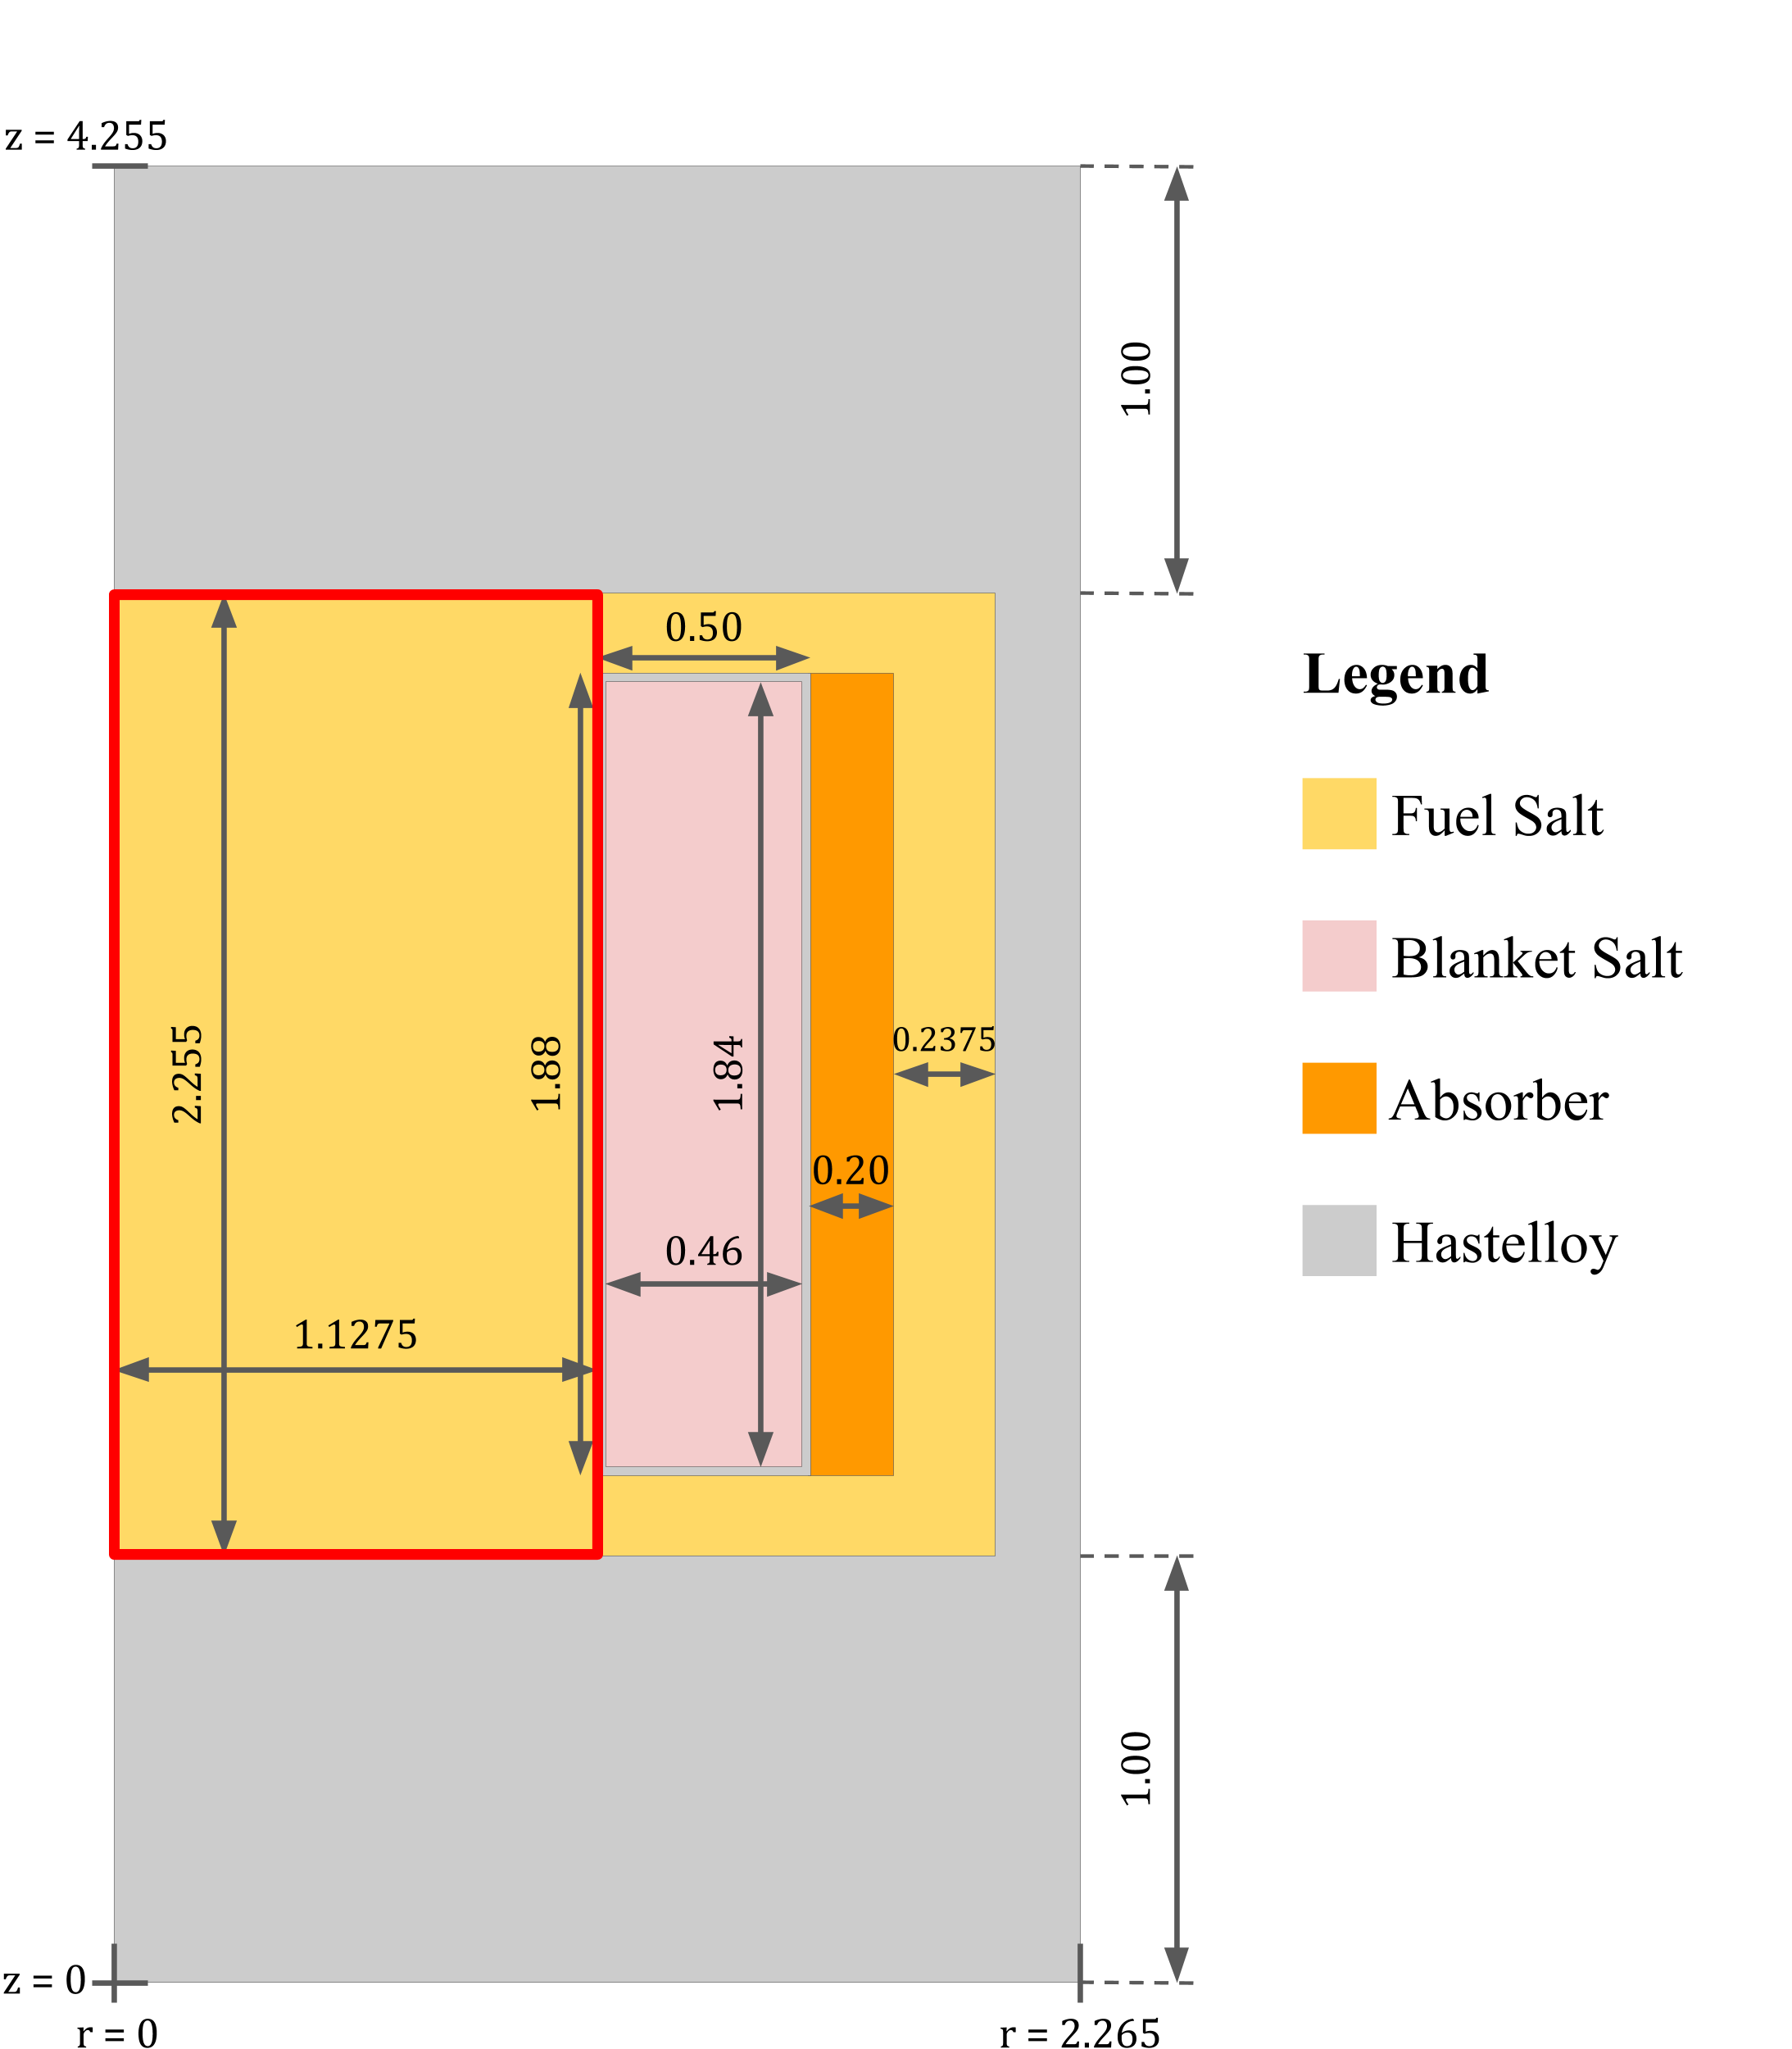
\includegraphics[width=.75\textwidth]{central-core-legend}
    \caption{2-D axisymmetric model of the MSFR. The red box indicates the
    central core region in the modeling approach in Moltres.}
    \label{fig:core}
\end{figure}

The central core region is of greatest interest to us during steady-state and
transient scenarios; the center of the reactor is naturally where most of the
fissions and heat generation occur.

\subsubsection{Neutronics Model}

Moltres performs neutron flux calculations in the central core region
using the standard formulations for the time-dependent multigroup
neutron diffusion equations and \gls{DNP} concentration equations as shown in
equations \ref{eq:neut} and \ref{eq:dnp}:
%
\begin{align}
    \frac{1}{v_g} \frac{\partial \phi_g}{\partial t} &= \nabla \cdot D_g
    \nabla \phi_g - \Sigma^r_g \phi_g +
    \sum^G_{g' \neq g} \Sigma^s_{g' \rightarrow g} \phi_{g'} + \chi^p_g
    \sum^G_{g'=1} (1-\beta) \nu \Sigma^f_{g'} \phi_{g'} + \chi^d_g \sum^I_i
    \lambda_i C_i, \label{eq:neut} \\
    \frac{\partial C_i}{\partial t} &= \beta_i \sum^G_{g'=1} \nu \Sigma^f_{g'}
    \phi_{g'} - \lambda_i C_i - \vec{u} \cdot \nabla C_i + \nabla \cdot
    K \nabla C_i, \label{eq:dnp} \\
    \intertext{where}
    v_g &= \text{average speed of neutrons in group $g$ [cm$\cdot$s$^{-1}$],} 
    \nonumber \\
    \phi_g &= \text{neutron flux in group $g$ [cm$^{-2}\cdot$s$^{-1}$],}
    \nonumber \\
    t &= \text{time [s],} \nonumber \\
    D_g &= \text{diffusion coefficient of neutrons in group $g$
    [cm$^2\cdot$s$^{-1}$],} \nonumber \\
    \Sigma^r_g &= \text{macroscopic cross section for removal of neutrons from
    group $g$ [cm$^{-1}$],} \nonumber \\
    \Sigma^s_{g' \rightarrow g} &= \text{macroscopic cross section of
    scattering from $g'$ to $g$ [cm$^{-1}$],} \nonumber \\
    \chi^p_g &= \text{prompt fission spectrum for neutrons in group $g$ [ - ],
    } \nonumber \\
    G &= \text{total number of discrete neutron groups [ - ],} \nonumber \\
    \nu &= \text{average number of neutrons produced per fission [ - ],}
    \nonumber \\
    \Sigma^f_{g} &= \text{macroscopic fission cross section for neutron in
    group $g$ [cm$^{-1}$],} \nonumber \\
    \chi^d_g &= \text{delayed fission spectrum for neutrons in group $g$
    [ - ],} \nonumber \\
    I &= \text{total number of delayed neutron precursor groups [ - ],}
    \nonumber \\
    \beta &= \text{total delayed neutron fraction [ - ],} \nonumber \\
    \beta_i &= \text{delayed neutron fraction of precursor group $i$ [ - ],}
    \nonumber \\
    \lambda_i &= \text{average decay constant of delayed neutron precursors in
    precursor group $i$ [s$^{-1}$],} \nonumber \\
    C_i &= \text{concentration of delayed neutron precursors in precursor
    group $i$ [cm$^{-3}$],} \nonumber \\
    K &= \text{turbulent diffusion coefficient of the delayed neutron
    precursors [cm$^2\cdot$s$^{-1}$].} \nonumber
\end{align}
%

While the limitations of the multigroup neutron diffusion method compared to
other deterministic and Monte Carlo methods, particularly for flux values near
boundaries, are well-documented, the diffusion model provides acceptable
accuracy at lower computational costs. Moreover, the central core region
contains no material interfaces except at its boundaries. Chapter
\ref{chap:nts} provides a comparison of the \gls{MSFR} multiplication factor
values and reactivity coefficients between Moltres and Serpent.

The \gls{DNP} concentration equation has additional advection and turbulent
diffusion terms to account for the movement of \glspl{DNP} in the primary
coolant loop. The turbulent diffusion $K$ is governed by the following
equation:
%
\begin{align}
    K &= \frac{\mu_t}{\rho Sc_t}
    \intertext{where}
    \mu_t &= \text{ eddy viscosity [Pa s],} \nonumber \\ 
    \rho &= \text{ density of the fuel salt [kg m$^{-3}$],} \nonumber \\
    Sc_t &= \text{ turbulent Schmidt number [ - ].} \nonumber
\end{align}
%
This work assumes $Sc_t = 0.85$ for a fair comparison with the Polimi and
TUDelft models \cite{fiorina_modelling_2014} which used the same value. It has
its roots in the Reynolds Analogy, which states that turbulent momentum and
heat transfer largely depend on the same eddies in turbulent flow
\cite{bartosiewicz_612_2019}. Therefore,
$Sc_t$ should be close to unity. $Sc_t = 0.85$ is also the default value for
most commercial \gls{CFD} software \cite{bartosiewicz_612_2019}.

\begin{figure}[htb!]
    \centering
    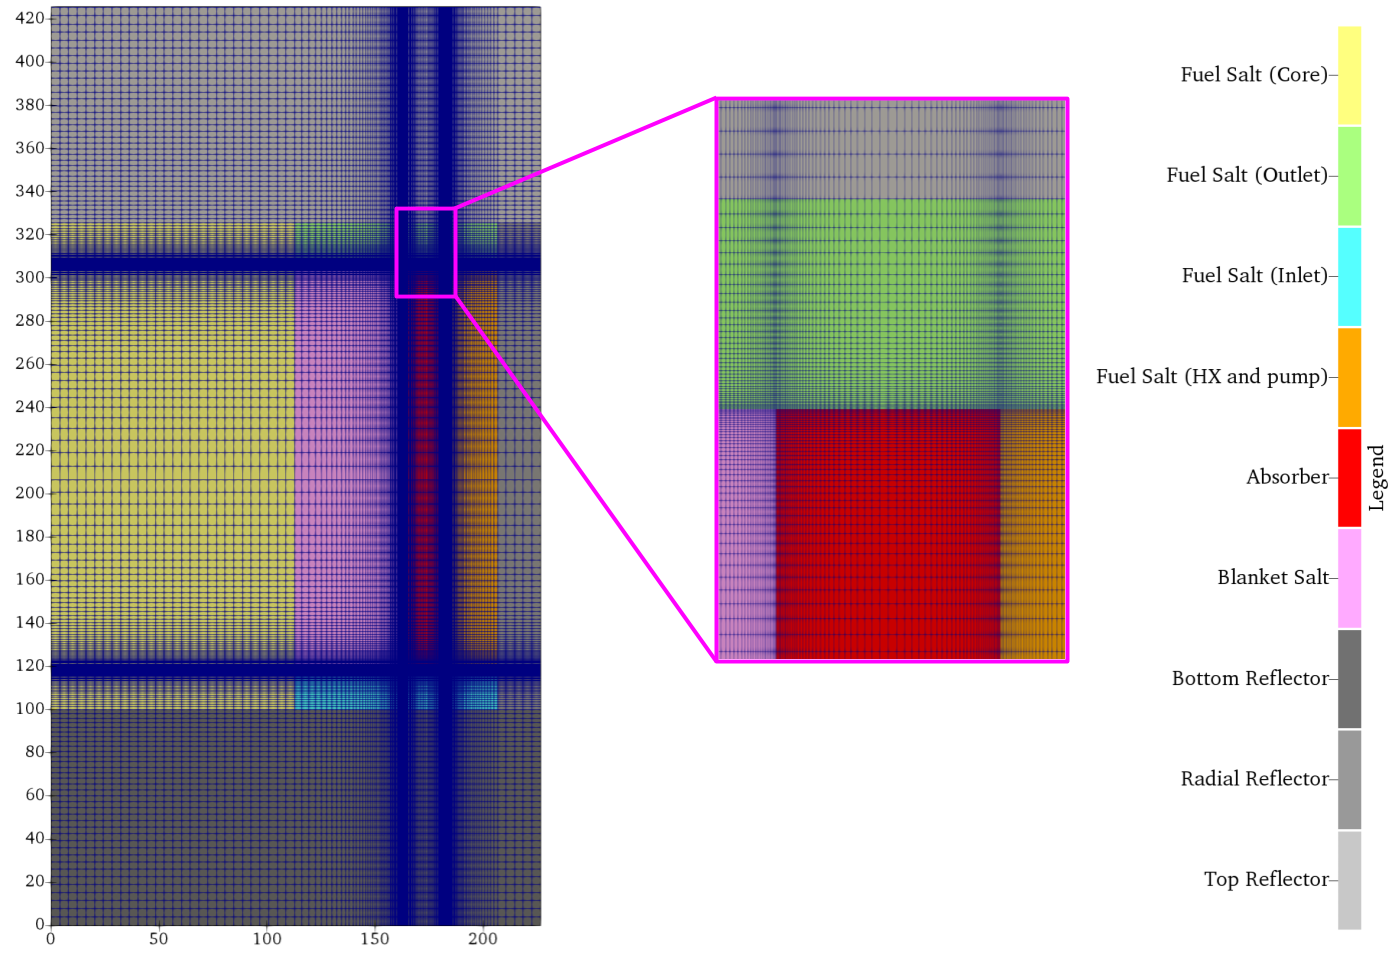
\includegraphics[width=\textwidth]{mesh2}
    \caption{Mesh adopted in Moltres and a close-up view of the mesh around
    the boron carbide absorber.}
    \label{fig:mesh}
\end{figure}

Moltres users can use an arbitrary number of neutron energy groups as
long as they provide Moltres with the appropriate group constant data. The
number of precursor groups is also variable, though usually predetermined by
the choice of nuclear data library in the group constant generation step.
Moltres automatically interpolates the group constant data for required
temperatures using one of the many predefined interpolation methods available
in \gls{MOOSE}. Once again, Moltres allows users to select their
interpolation method of choice.

This work uses six neutron energy groups according to the
energy boundaries in table \ref{table:bound}, and eight \gls{DNP} groups as
defined by the JEFF-3.1.2 library. The neutron flux
and \gls{DNP} concentration values were approximated by first-order Lagrange
and constant monomial shape functions respectively on the finite element mesh.
Figure \ref{fig:mesh} shows the mesh adopted for the \gls{MSFR} model.
This work assumes vacuum boundary conditions for all six neutron group fluxes
along the external boundaries of the geometry, and homogeneous Neumann
boundary conditions along the axial symmetry boundary. For the \gls{DNP}
concentrations, this work imposed homogeneous Neumann boundary conditions on
the walls, and inflow and outflow boundary conditions on the inlet and outlet
boundaries, respectively. The inlet \gls{DNP} concentration values were
imported from the outlet values of the 1-D outer loop pipe at the same
timestep. Table \ref{table:corebc} describes these boundary conditions
mathematically.

For the decay heat model, a previous study on the MSFR by Aufiero et al.
\cite{aufiero_extended_2013} showed that using three decay heat precursor
groups with appropriate half-lives in the form of exponential equations, can
accurately model decay heat in the MSFR for up to 300 seconds after shutdown
with a relative error of less than 2\%. Thus, this thesis implements the new
decay heat modeling capability with the following equation:
%
\pagebreak
\begin{align}
	\frac{\partial \omega_j}{\partial t} &= f_j \lambda_j \sum^G_{g=1}
	\epsilon_{g}
	\Sigma^f_{g} \phi_{g} - \lambda_j \omega_j - \vec{u} \cdot \nabla
	\omega_j + \nabla \cdot K \nabla \omega_j, \label{eq:decayheat} \\
	\intertext{where}
    \omega_j &= \text{total decay heat power density from decay heat
    precursors in group $j$ [W$\cdot$cm$^{-3}$],} \nonumber \\
	f_j &= \text{fraction of total power attributable to decay heat group
	$j$ [ - ],} \nonumber \\
	\epsilon_g &= \text{average fission energy per fission initiated by a
	neutron in group $g$ [W],} \nonumber \\
	\lambda_j &= \text{average decay constant of decay heat precursors in
	group $j$ [s$^{-1}$].} \nonumber
\end{align}

Like the neutron energy and \gls{DNP} groups, Moltres can accommodate an
arbitrary number of decay heat groups. The current work uses the same decay
heat fractions and decay constants, shown in Table \ref{eq:decayheat}, used in
the Polimi and TUDelft models for three decay heat groups.

\begin{table}[htb!]
	\centering
	\caption{Decay heat group parameters \cite{fiorina_modelling_2014}.}
	\begin{tabular}{S S S}
		\toprule
		{Decay heat group $j$} & {$\lambda_j$ [s$^{-1}$]} & {$f_j$} \\
		\midrule
		1 & 0.1974 & 0.0117 \\
		2 & 0.0168 & 0.0129 \\
		3 & 0.000358 & 0.0186 \\
		\bottomrule
	\end{tabular}
	\label{table:decayheat}
\end{table}

\subsubsection{Thermal-Hydraulics Model}

This work models fluid dynamics using the \gls{INS} capabilities from the
MOOSE Navier-Stokes module \cite{peterson_overview_2017}. The standard
\gls{INS} equations are:
%
\begin{align}
    \text{Momentum eq.:} && \rho \frac{\partial \vec{u}}{\partial t} &=
    -\rho (\vec{u}
    \cdot \nabla) \vec{u} + \nabla \cdot [-p \vec{I} + \mu [
    \nabla \vec{u} + (\nabla \vec{u})^T]] + \vec{f} &&
    \label{eq:momemtum} \\
    \text{Divergence-free:} && \nabla \cdot \vec{u} &= 0 &&
    \label{eq:divergence}
    \intertext{where}
    && p &= \text{ pressure [Pa],} && \nonumber \\
    && \mu &= \text{ dynamic viscosity [Pa$\cdot$s],} && \nonumber \\
    && \vec{f} &= \text{ body force per unit volume [N$\cdot$m$^{-3}$].} &&
    \nonumber
\end{align}

In addition to the intrinsic molecular viscosity in the \gls{INS} equations,
this thesis includes an eddy viscosity term, $\mu_t$, to approximate
turbulent flow effects. The current implementation of the Navier-Stokes module
does not have a turbulence model. The options for turbulence modeling in
\gls{CFD} include direct numerical simulations (DNS) and large eddy
simulations (LES) for higher fidelity flow simulations, \gls{RANS} methods for
balanced compromises between accuracy and computational speed, and lumped
parameter and sub-channel methods for even faster performance with greater
accuracy costs \cite{moorthi_review_2018}. The Polimi and TUDelft models used
\gls{RANS} methods to model salt flow \cite{fiorina_modelling_2014}. This work
uses a zeroth-order approximation of $\mu_t$ based on the calculated $\mu_t$
values reported in the Polimi and TUDelft models. The models predicted spatial
$\mu_t$ values ranging from 0 to 110 Pa$\cdot$s, with most values
falling within the 30 to 50 Pa$\cdot$s range. Thus, the present work uses
the approximated value $\mu_t=$ 40 Pa$\cdot$s. Despite the simplicity of this
approximation, the resulting flow profile is similar to the flow profile in
the Polimi and TUDelft models at steady-state.

The energy balance equation for temperature used in this Moltres model is:
%
\begin{align}
    \rho c_{p} \frac{\partial T}{\partial t} &= - \rho c_p \vec{u}
    \cdot \nabla T + \nabla \cdot [(k + k_t) \nabla T] + Q_s
    \label{eq:temp} \\
    k_t &= \frac{\mu_t}{\rho Pr_t} \\
    Q_s &= \Big( 1 - \sum^J_{j=1} f_j \Big) \sum^G_{g=1} \epsilon_g \Sigma_g^f
    \phi_g + \sum^J_{j=1} \omega_j, \label{eq:source}
    \intertext{where}
    c_p &= \text{specific heat capacity of molten salt
    [J$\cdot$kg$^{-1}\cdot$K$^{-1}$],} \nonumber \\
    T &= \text{temperature of molten salt [K]} \nonumber \\
    \vec{u} &= \text{velocity of molten salt [m$\cdot$s$^{-1}$],}
    \nonumber \\
    k &= \text{thermal conductivity of molten salt
    [W$\cdot$m$^{-1}\cdot$K$^{-1}$],} \nonumber \\
    J &= \text{total number of decay heat groups [ - ].} \nonumber
\end{align}
%
The diffusion term includes turbulent heat
diffusivity based on the eddy viscosity $\mu_t$ and the turbulent Prandtl
number $Pr_t$. $Pr_t$ is also 0.85 due to the same reasoning provided for
$Sc_t$. The first term in the heat source $Q_s$ equation represents prompt
fission heat, and the second term represents decay heat from the $J$ decay
heat groups.

With this model, the results were expected to show good qualitative agreement
with the Polimi and TUDelft models, including the large recirculation region
near the blanket tank walls and the resulting high temperatures in that
region. The results in Chapter \ref{chap:ss} show minor discrepancies in
regions where the viscosity values were under- or over-predicted.

\subsubsection{Boundary Conditions}

Table \ref{table:corebc} summarizes the boundary conditions for all variables
on all of the relevant boundaries. Figure \ref{fig:msfrbc} shows the locations
of the various boundaries listed in the table. The CoupledOutflow boundary
condition for $C_i$ and $\omega_j$ is a new feature in Moltres that allows
users to couple these variables to the outlet velocity components (e.g. $u_x$,
$u_y$). Without this boundary condition, users could only use uniform or fixed
function-based velocity profiles in conjunction with the precursor looping
capability.

\begin{table}[htbp!]
    \small
	\caption{Boundary conditions in the main reactor geometry (Figure
	\ref{fig:msfrbc}).}
	\centering
	\begin{tabular}{ l l c}
		\toprule
		Variable & Boundary & Boundary Condition \\
		\midrule
		\multirow{4}{*}{Neutron flux $\phi_g$} & Top & $\frac{d \phi_g}{dx}
		\big|_{\text{inflow}} = 0$ \\[.5ex]
        & Outer & $\frac{d \phi_g}{dx} \big|_{\text{inflow}} = 0$ \\[.5ex]
        & Bottom & $\frac{d \phi_g}{dx} \big|_{\text{inflow}} = 0$ \\[.5ex]
        & Axial & $\frac{d \phi_g}{dx} = 0$ \\[.5ex]
        \midrule
        \multirow{6}{*}{Delayed neutron precursor concentration $C_i$} &
        Top (Core) & $\frac{d C_i}{dx} = 0$ \\[.5ex]
        & Bottom (Core) & $\frac{d C_i}{dx} = 0$ \\[.5ex]
        & Outer (Core) & $\frac{d C_i}{dx} = 0$ \\[.5ex]
        & Axial (Core) & $\frac{d C_i}{dx} = 0$ \\[.5ex]
        & Inlet (Core) & $C_i = c$ \\
        & Outlet (Core) & $u_x \cdot C_i = 0$ \\
        \midrule
        \multirow{6}{*}{Decay heat power density $\omega_j$} &
        Top (Core) & $\frac{d \omega_j}{dx} = 0$ \\[.5ex]
        & Bottom (Core) & $\frac{d \omega_j}{dx} = 0$ \\[.5ex]
        & Outer (Core) & $\frac{d \omega_j}{dx} = 0$ \\[.5ex]
        & Axial (Core) & $\frac{d \omega_j}{dx} = 0$ \\[.5ex]
        & Inlet (Core) & $\omega_j = c$ \\
        & Outlet (Core) & $u_x \cdot \omega_j = 0$ \\
        \midrule
        \multirow{6}{*}{Radial velocity $u_x$} & Top (Core) & $u_x = 0$ \\
        & Bottom (Core) & $u_x = 0$ \\
        & Outer (Core) & $u_x = 0$ \\
        & Axial (Core) & $u_x = 0$ \\
        & Inlet (Core) & $u_x = c$ \\
        & Outlet (Core) & $\frac{d u_x}{dx} = 0$ \\[.5ex]
        \midrule
        \multirow{6}{*}{Axial velocity $u_y$} & Top (Core) & $u_y = 0$ \\
        & Bottom (Core) & $u_y = 0$ \\
        & Outer (Core) & $u_y = 0$ \\
        & Axial (Core) & $\frac{d u_y}{dx} = 0$ \\[.5ex]
        & Inlet (Core) & $u_y = 0$ \\
        & Outlet (Core) & $\frac{d u_y}{dx} = 0$ \\[.5ex]
        \midrule
        \multirow{6}{*}{Temperature $T$} & Top (Core) &
        $\frac{d T}{dx} = 0$ \\[.5ex]
        & Bottom (Core) & $\frac{d T}{dx} = 0$ \\[.5ex]
        & Outer (Core) & $\frac{d T}{dx} = 0$ \\[.5ex]
        & Axial (Core) & $\frac{d T}{dx} = 0$ \\[.5ex]
        & Inlet (Core) & $T = c$ \\
        & Outlet (Core) & $\frac{d T}{dx} = 0$ \\[.5ex]
		\bottomrule
	\end{tabular}
	\label{table:corebc}
\end{table}

\clearpage

\begin{figure}[htb!]
    \centering
    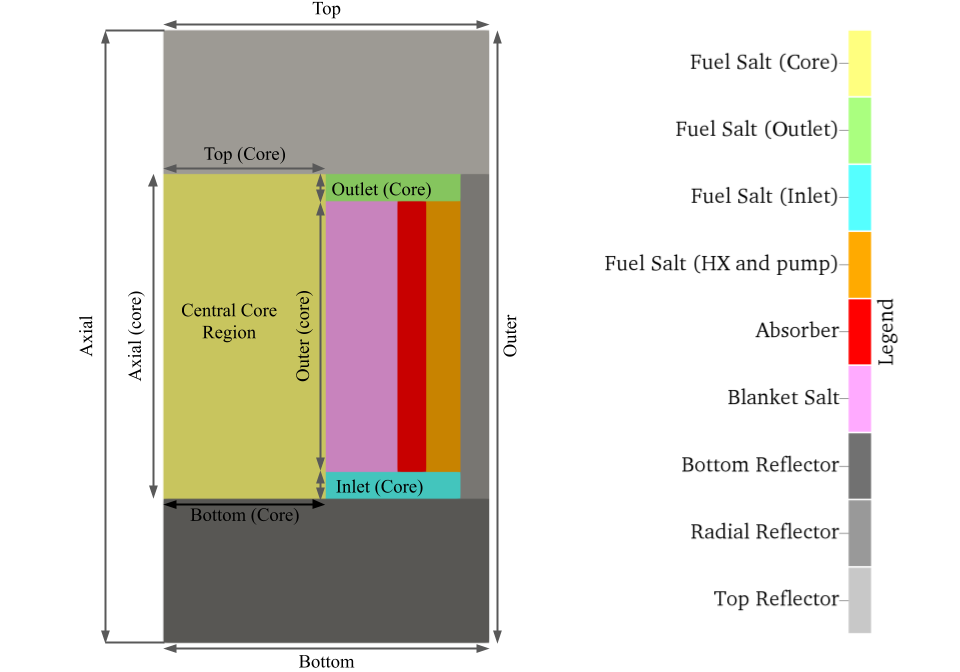
\includegraphics[width=.8\textwidth]{msfrbc}
    \caption{The boundaries in the \gls{MSFR} geometry that are relevant for
    the boundary conditions mentioned in Table \ref{table:corebc}.}
    \label{fig:msfrbc}
\end{figure}

\subsection{Outer Loop Region}

Moltres also accounts for the decay of
\glspl{DNP} outside the central core region by simulating its flow in a
separate 1-D pipe geometry. This outer loop pipe calculation is implicitly
coupled to the active core simulation through Picard iterations in MOOSE's
MultiApp functionality and inlet/outlet boundary values. For this work with
the \gls{MSFR} model, the pipe length is 2.255 m with salt flowing at 1.1275 m
s$^{-1}$ for an out-of-core residence time of 2 s. The present author derived
these parameters from the reference specifications of 4s cycle
time and 50\% out-of-core salt fraction (Table \ref{table:msfr}).

\subsubsection{Neutronics Model}

The outer loop region is largely subcritical because most of it is adjacent to
the boron carbide absorber as shown in Figure \ref{fig:core}. Therefore, the
only significant neutronics-related phenomena are the drift and decay of
\glspl{DNP}. The governing equation for the \glspl{DNP} is:
%
\begin{align}
    \frac{\partial C_i}{\partial t} &= - \lambda_i C_i - u
    \frac{\partial C_i}{\partial x}.
    \label{eq:dnploop}
\end{align}
%
Equation \ref{eq:dnploop} is derived from equation \ref{eq:dnp} by removing
the fission \gls{DNP} source term, and the conversion of the advection and
diffusion terms to their 1-D forms. The decay constants and diffusion
coefficient are the same values used in the central core region.

\subsubsection{Thermal-Hydraulics Model}

A constant velocity of 1.1275 m s$^{-1}$ is applied in the outer loop region
to maintain the nominal 2s out-of-core residence time. The governing equation
for temperature, derived from equation \ref{eq:temp}, is:
%
\begin{align}
    \rho c_{p} \frac{\partial T}{\partial t} &= - \rho c_p u
    \frac{\partial T}{\partial x} - Q_{hx} \label{eq:temploop} \\
    Q_{hx} &= \alpha (T - T_i) \delta (x_0) \label{eq:hx} \\
    \intertext{where}
    Q_{hx} &= \text{heat removal rate through the heat exchanger [W],} 
    \nonumber \\
    \alpha &= \text{heat transfer coefficient [W$\cdot$K$^{-1}$],} \nonumber
    \\
    T_i &= \text{temperature of the intermediate salt [K],} \nonumber \\
    x_0 &= \text{position of the point heat exchanger [m].} \nonumber
\end{align}

In the outer loop region, the fission heat source term is replaced with a heat
exchanger sink term $Q_{hx}$
which depends on the temperature difference between the fuel salt $T$ and the
intermediate loop salt $T_i$. For simplicity, this work assumes a constant
temperature of 823 K in the intermediate loop. The heat transfer coefficient
was determined by assuming that the fuel outlet temperature is 1023 K and
calculating the heat removal rate to induce a 100 K drop at the given
volumetric flow rate and heat capacity of the fuel salt. The resulting value
for $\alpha$ is 370.668 W$\cdot$K$^{-1}$. This work opted to
ignore the diffusion term due to the discontinuity of the temperature
distribution across the point heat exchanger. 

\subsubsection{Boundary Conditions}

Table \ref{table:loopbc} summarizes the boundary conditions for all variables
on the inlet and outlet of the 1-D outer loop region. The inlet boundary
conditions are all Dirichlet boundary conditions. The inlet boundary values
are set by the outflow from the central core region that this inlet is
connected to in the actual reactor geometry. The outlet boundary conditions
are all outflow boundary conditions as shown in Table \ref{table:loopbc}.

\begin{table}[htbp!]
    \small
	\caption{Boundary conditions in the 1-D outer loop geometry. $u$
	represents the 1-D velocity in this region.}
	\centering
	\begin{tabular}{ l l c}
		\toprule
		Variable & Boundary & Boundary Condition \\
        \midrule
        \multirow{2}{*}{Delayed neutron precursor concentration $C_i$} &
        Inlet (Core) & $C_i = c$ \\
        & Outlet (Core) & $u \cdot C_i = 0$ \\
        \midrule
        \multirow{2}{*}{Decay heat power density $\omega_j$} &
        Inlet (Core) & $\omega_j = c$ \\
        & Outlet (Core) & $u \cdot \omega_j = 0$ \\
        \midrule
        \multirow{2}{*}{Temperature $T$} &
        Inlet (Core) & $T = c$ \\
        & Outlet (Core) & $u \cdot T = 0$ \\
		\bottomrule
	\end{tabular}
	\label{table:loopbc}
\end{table}

\subsection{Central Core and Outer Loop Coupling}

This subsection details the delayed neutron and decay heat precursors, and
temperature coupling between the central core and outer loop regions. 

%Starting with the central core region, for the neutron group fluxes, we
%imposed vacuum boundary conditions on the
%outermost boundaries of the geometry in Figure \ref{fig:core} excluding the
%axial boundary. The \gls{DNP} variables have homogeneous Neumann boundary
%conditions along the axis and the walls in the central core region, and inflow
%and outflow boundary conditions on the inlet and outlet boundaries,
%respectively. The temperature variable shares the same type of boundary
%conditions as the \gls{DNP} variables.

This work uses a parabolic flow profile on the inlet Dirichlet boundary
condition. The equation for $u_x$ at the inlet is:
%
\begin{align}
    u_x &= -\xi \Big[\frac{y}{H} - \Big(\frac{y}{H}\Big)^2 
    \Big] \\
    \intertext{where}
    \xi &= \text{normalizing constant [m$\cdot$s$^{-1}$],} \nonumber \\
    y &= \text{height along the inlet [m],} \nonumber \\
    H &= \text{total height of the inlet $= 0.1875$ m.} \nonumber
\end{align}
%
$\xi$ is a normalizing constant that depends on the total volumetric flow
rate, $\dot{V}$. Solving the following set of equations in $v$ and $\dot{V}$:
%
\begin{align}
    v &= \xi [\frac{y}{H} - \frac{y^2}{H^2}] \\
    \dot{V} &= \int^h_0 \int^{2 \pi}_0 v r d\theta dy \\
    \intertext{where}
    r &= \text{radius [m],} \nonumber \\
    \theta &= \text{azimuthal angle [rad],} \nonumber
\end{align}
%
gives $\xi = 20.3401$ m$\cdot$s$^{-1}$ for $\dot{V} = 4.5$ m$^3\cdot$s$^{-1}$. 

At every timestep, Moltres also calculates weighted averages of the
temperature and the precursors at the outlet. These values are weighted by the
outflow velocity values at the outlet according to the following equation:
%
\begin{align}
    \overline{\psi} &= \frac{\int_\mathcal{C} \psi(y) u(y) dy}{
    \int_\mathcal{C} u(y) dy} \\
    \intertext{where}
    \psi &= \text{variable to be weighted [ - ]} \nonumber \\
    \mathcal{C} &= \text{outlet boundary area [ - ]} \nonumber \\
    u &= \text{outflow velocity perpendicular to the outlet boundary
    [m$\cdot$s$^{-1}$].} \nonumber
\end{align}

Moltres transfers this outflow value from the central core region to the 1-D
outer loop region, to be used as the boundary value for the inhomogeneous
Dirichlet boundary
condition at the inlet. Likewise, the outflow value from the outer
loop region is used for the inflow value in the central core region. No
averaging is required for this step as the outer loop region is a 1-D system.
We assume that the inflow temperature and \gls{DNP} are uniform at the inlet.
The Picard iterations within every timestep ensure that the two systems are
implicitly coupled even though they're solved separately.


\chapter*{Appendix}
Appendix.

\backmatter

\bibliographystyle{ieeetr}
\bibliography{bibliography}

\end{document}
\endinput
%%
%% End of file `thesis-ex.tex'.
